%!TEX root = ../main.tex
\doublespacing
\chapter{Theoretical Background}
\label{chap:theory}
The following chapter describes the core concepts relevant to this thesis in more detail than Chapter \ref{chap:intro}. Here I discuss the various mechanisms for radio wave emission in the solar corona, with particular emphasis on the plasma emission process. I will also give an introduction to the mathematical formalisms of radio interferometry.
\section{Introductory Concepts in Plasma Physics}
Plasma was the name given by Langmuir to the new, exotic type of matter he was studying in the 1920s. It is essentially an ionized gas that exhibits quasi-neutrality on a macroscopic scale. The solar corona is a shell of hot plasma surrounding the Sun and as such, the study of emission from the corona is a study of the plasma itself. A plasma's tendency to remain in quasi-neutrality means that any change to the charge separation between electrons and ions generates an electric field which acts as a restoring force and thus oscillations are induced in the plasma. To determine the frequency of these oscillations imagine the following, a plasma with equal number density of electrons and ions $N_e = N_i = N_0$ is perturbed so that a group of electrons are moved by some distance $x$ a restoring force $\mathbf{E} = q_e E_x$ acts to bring the electrons back to their initial position. Due to their mass, the electrons overshoot their initial position and the process begins again in the opposite direction. Here we have made the safe assumption that, due to electrons being much lighter, the ions remain stationary. For electrons with mass $m_e$, Newton's second law gives us,
\begin{equation}
\label{eq:fma}
m_e \frac{d^2x}{dt^2} = q_e E_x.
\end{equation}
Guass' law for some closed, rectangular box surface, $S$, inside our perturbed plasma gives, 
$$
\oint_S \mathbf{E} \cdot d\mathbf{s} = \frac{Q}{\epsilon_0}
$$
where $Q$ is the total charge contained within the closed surface $S$. Given the equilibrium density of electrons, $N_e$, the total charge must be $Q = A x N_e q_e$ where $A$ is the cross-sectional area of $S$. For $A=a\Delta z$, we can solve for  $E_x$ to find,
$$
\oint_S \mathbf{E} \cdot d\mathbf{s} = -a \Delta z E_x =  \frac{Q}{\epsilon_0} = \frac{ax\Delta z N_e q_e}{\epsilon_0} \rightarrow E_x = -\frac{x N_e q_e}{\epsilon_0}.
$$
Using this with Equation \ref{eq:fma} we obtain the ordinary differential equation,
\begin{equation}
\label{plasma_motion}
m_e \frac{d^2 x}{dt^2} + \frac{N_e q_e^2}{\epsilon_0} x = 0 \rightarrow \frac{d^2 x}{dt^2} + \omega_p^2 x = 0.
\end{equation}
The solution to this equation is the well known harmonic oscillator with an angular frequency $\omega_p$ which we call the electron plasma frequency or simply, the plasma frequency
\begin{equation}
\label{eq:plasma_freq}
\omega_p = \sqrt{\frac{N_e q_e^2}{\epsilon_0 m_e}}.
\end{equation}
The plasma frequency leads us to an important criterion that a partially ionised gas must have to be considered a plasma. That is, plasma oscillations can only develop if the mean free time between collisions of electrons and ions with neutrals, $\tau_n$, is longer than the oscillation period $\tau_p = 1/ \omega_p$, or $\omega_p \tau_n >1$.

Another implication of the quasi-neutrality of plasmas can be seen when one considers immersing a test particle of charge $Q_+$ inside an initially uniform plasma at time $t = 0$ such that, again, $N_i = N_e = N_0$. The electric potential in the plasma is that due to the single test charge, 
$$
\Phi (\mathbf{r}) = \frac{1}{4 \pi \epsilon_0} \frac{Q}{r},
$$
assuming the test charge is at the origin of our spherical coordinate system. Once again we assume that because the ions are much more massive compared to the electrons in the plasma that their motion can be neglected. The electrons in the plasma are attracted to the test charge causing the electron density near the test charge to increase. The new potential distribution $\Phi (\mathbf{r})$ must be re-evaluated using Poisson's equation:
\begin{equation}
\label{eq:test_charge}
\nabla^2 \Phi (\mathbf{r}) = - \frac{\rho}{\epsilon_0} = - \frac{q_e(N_e - N_i)}{\epsilon_0},
\end{equation}
where the excess free charge density near the test charge is $\rho = q_e (N_e - N_i)$. In spherical coordinates this leads to an electron density distribution of,
\begin{equation}
\label{eq:e_density}
N_e(r) = N_0 e^{-q_e \Phi (r)/k_b T_e}
\end{equation}
where $k_B$ is Boltzman's constant and $T_e$ is the electron temperature. Subbing into the spherical coordinate version of Equation \ref{eq:test_charge} gives,
\begin{equation}
\label{eq:spherical_poisson}
\frac{1}{r^2} \frac{d}{dr}\left(r^2 \frac{d \Phi}{dr} \right) = - \frac{q_e N_0}{\epsilon_0}\left[\exp\left(\frac{-q_e \Phi (r)}{k_BT}\right) -1 \right],\  r>0.
\end{equation}
Assuming $\vert q_e \Phi \vert \ll k_b T$, Equation \ref{eq:spherical_poisson} can be expanded as a power series to give, 
$$
\frac{1}{r^2} \frac{d}{dr}\left(r^2 \frac{d \Phi}{dr} \right) \simeq \left[ \frac{N_0q_e^2}{\epsilon_0 k_B T_e} \right]\Phi (r) = \frac{1}{\lambda_D^2}\Phi(r)
$$
where $\lambda_D$, known as the Debye length, is defined to be
\begin{equation}
\label{eq:debye_length}
\lambda_D = \sqrt{\frac{\epsilon_0 k_B T_e}{N_0 q_e^2}}.
\end{equation}
The solution to the above can be found to be 
\begin{equation}
\label{eq:phi_solution}
\Phi (r) = \left[ \frac{1}{4 \pi \epsilon_0} \frac{Q}{r}\right] e^{-r/\lambda_D},
\end{equation} 
which shows that for $r \gg \lambda_D$, the potential of the test charge disappears. Thus the Debye length of a plasma can be used to define a second plasma criterion: an ionised gas can only be considered a plasma if the length scale of the system, $L$, is much greater than the Debye length.
\subsection{Kinetic Theory}
Armed with some knowledge of fundamental plasma behaviour, we jump forward through plasma theory to determine the collective properties of plasmas using averages over large numbers of particles. In order to do so, the positions and velocities of plasma particles are described using a distribution function in what is called plasma kinetic theory. We start without worrying about the exact form of this distribution function and instead assume that the position of each particle in our plasma is given by a vector $\mathbf{r}$ from the origin where,
\begin{equation}
\label{eq:KT_position}
\mathbf{r} = \mathbf{\hat{x}}x + \mathbf{\hat{y}}y + \mathbf{\hat{z}}z
\end{equation}
and that each particle has a linear velocity,
\begin{equation}
\label{eq:KT_velocity}
\mathbf{v} = \mathbf{\hat{x}}v_x + \mathbf{\hat{y}}v_y + \mathbf{\hat{z}}v_z
\end{equation}
so that the particle speed is $\vert \mathbf{v} \vert = v = \sqrt{v_x^2 + v_y^2 + v_z^2}$. Thus, at any given time, the position and velocity of a particle can be represented as a point in a six dimensional phase space determined by the coordinates $x, y, z, v_x, v_y$ and $v_z$. Now consider a volume element $d\mathbf{r} = d^3r = dxdydz$ such that it is large enough to contain a great number of particles but small enough so that macroscopic quantities vary only slightly inside it. Also consider a time interval $dt$ centred around time $t$, where $dt$ is long compared to the mean time for a particle to traverse $d\mathbf{r}$ but similarly short enough compared to the time scales of the macroscopic parameters of the plasma. The number of particles in $d\mathbf{r}$ averaged over $dt$ is simply $N(\mathbf{r},t)d\mathbf{r}$ where $N(\mathbf{r},t)$ is the number density of particles. In the same manner, one can define a density of the number of particles in velocity space which we denote as $f(\mathbf{r}, \mathbf{v}, t)d\mathbf{r}$. From this, we can determine the number of particles at time $t$ in the element $d\mathbf{r}$ and with velocities between $\mathbf{v}$ and $\mathbf{v} + d\mathbf{v}$ is $f(\mathbf{r}, \mathbf{v}, t)d\mathbf{r}d\mathbf{v}$ The function $f(\mathbf{r}, \mathbf{v}, t)$ is called the velocity distribution function and is the density of representative points in phase space. The total number of velocity points in all of velocity space can be found by summing the number of velocity points $f(\mathbf{r}, \mathbf{v}, t)d\mathbf{r}d\mathbf{v}$ in $d\mathbf{v}$ over all possible velocities. Following from this, we can obtain the number density of particles:
\begin{equation}
\label{eq:KT_number_density}
N(\mathbf{r},t) =\int^\infty_{-\infty}  f(\mathbf{r}, \mathbf{v}, t) d\mathbf{v}.
\end{equation}

Other macroscopic plasma parameters (e.g. mass density, flux, current) can be obtained using the velocity distribution function. Consider any property $g(\mathbf{r},\mathbf{v}, t)$ of a particle. The average value of this quantity is given by
\begin{equation}
\label{eq:KT_average_value}
g_{\mbox{av}}(\mathbf{r}, t)  = \langle g(\mathbf{r}, \mathbf{v}, t) \rangle = \frac{1}{N(\mathbf{r}, t)} \int g(\mathbf{r}, \mathbf{v}, t) f(\mathbf{r}, \mathbf{v}, t) d\mathbf{v}.
\end{equation}
The evolution of the velocity distribution function, which we henceforth refer to as the distribution function, or $f$, in time is determined by the Boltzmann Equation:
\begin{equation}
\label{eq:KT_Boltzmann_eq}
\frac{\partial f}{\partial t} + (\mathbf{v} \cdot \nabla_\mathbf{r})f + \left[ \left(\frac{\mathbf{F}}{m} \right) \cdot \nabla_\mathbf{v}\right]f = \left( \frac{\partial f}{\partial t} \right)_{\mbox{coll}}
\end{equation}
where $\mathbf{F} =m\mathbf{a}$ is a force acting on the particles.
The Boltzmann equation is essentially a statement on the conservation of points in phase space. The left hand side describes particle flow through the volume element $d\mathbf{r} d\mathbf{v}$ and it is balanced by the collisional term on the right hand side. By considering a homogeneous plasma in a steady-state (i.e. in thermal equilibrium) with no external forces, the terms on the left hand side of the Boltzmann equation all become 0 and thus 
$$
\left( \frac{\partial f}{\partial t} \right)_{\mbox{coll}} = 0.
$$
By considering the particle collisions in which energy must be conserved under the above assumptions it can be shown that the distribution function takes the form of the Maxwell-Boltzmann distribution:
\begin{equation}
\label{eq:KT_maxwellboltzmann}
f(\mathbf{r}, \mathbf{v}, t) = f(v) = N_0 \left( \frac{m}{2 \pi k_B T} \right)^{\frac{3}{2}} e^{-mv^2/(2K_BT)}.
\end{equation}
By substituting the Lorentz force into \ref{eq:KT_Boltzmann_eq}, assuming no collisions, gives the Vlasov equation:
\begin{equation}
\label{eq:KT_Vlasov_eq}
\frac{\partial f}{\partial t} + (\mathbf{v} \cdot \nabla_\mathbf{r})f + \frac{q}{m} \left[ \left(\mathbf{E} + \mathbf{v} \times \mathbf{B} \right) \cdot \nabla_\mathbf{v}\right]f = 0. 
\end{equation}
The Vlasov equation, together with Maxwell's equations for $\mathbf{E}$ and $\mathbf{B}$ represent a complete set of self-consistent equations to describe a plasma interacting with an electromagnetical field. So far we have considered the derivatives of $f$ with respect to a stationary reference frame. It is more convenient to consider a reference frame that moves with the fluid elements of a plasma. A derivative in this sense is known as a convective derivative or total time derivative and can be expressed for the distribution function as
\begin{equation}
\label{eq:KT_Vlasov_convective}
\frac{df}{dt} = \frac{\partial f}{\partial t} + (\mathbf{v} \cdot \nabla_\mathbf{r})f + \left(\frac{d\mathbf{v}}{dt} \cdot \nabla_\mathbf{v}\right)f.
\end{equation}
Thich has the interesting result that the collisionless Boltzmann equation can be written as
\begin{equation}
\label{eq:KT_Liouville}
\frac{df}{dt}=0,
\end{equation}
meaning that a particle moving through phase space will see a constant $f$ in its local frame. This is known as Liouville's theorem. The Boltzmann equation allows us to determine the macroscopic transport equations of a plasma, which will form the foundations of the theory in the section to come. This is done not by solving the Boltzmann equation itself but rather, multiplying it by various powers of $\mathbf{v}$ and integrating over velocity, i.e. ``taking the moments of the Boltzmann equation"
$$
\mu_n = \int \mathbf{v}^n\left[\mbox{Boltzmann Eq.}\right]dv,
$$
where $\mu_n$ is the $n$th order moment. This procedure gives up our knowledge on the velocity distribution of particles in order to instead obtain single-value macroscopic particles of a plasma fluid. The main results for the first 3 moments are shown here \footnote{The interested reader is referred to e.g. \cite{Inan2010} for a full derivation of these equations}:
\begin{align*}
\mu_0 \rightarrow  \mbox{continuity equation or conservation of mass} \\
\mu_1 \rightarrow  \mbox{momentum transport equation or conservation of momentum} \\
\mu_2 \rightarrow  \mbox{energy transport equation or conservation of energy}
\end{align*}
The moments of the Boltzmann equation allows us to develop the theory of plasmas as being made up of multiple fluids each of their different particle species, e.g. electrons and ions. Under certain conditions it is possible to consider the entire plasma as a single fluid and it is this approach, called magnetohydrodynamics, that I discuss next \footnote{The derivations of the equations of motion for a two-fluid plasma and their subsequent combination to a single fluid are complex and tedious. I therefore once again refer an interested reader to e.g. \cite{Inan2010}}.
\subsection{Magnetohydrodynamics}
\section{The Plasma Emission Mechanism for Type III Radio Bursts}
\label{sec:plasma}
In 1942 while Britain was on the look out for radar signals of enemy aircraft, a strong, noise like and highly variable signal was noticed by radar operators. Initially it was thought that Germany had managed to learn the secret of radar and create some sort of jamming device. On further investigation it was found that this jamming was in fact radio emission from the Sun. The discovery of this radio emission being associated with a major solar flare was kept secret until after the war and was published by \cite{Appleton1946}.
Since then a number of major advancements in both instrumentation and theory have occurred. A culmination of the theory of solar radio emission is laid out in the book by \cite{McLean1985} while worldwide, a number of extraordinary radio telescopes and interferometers such as the LOw Frequency ARray \cite[LOFAR,][]{VanHaarlem2013}, the Nan\c{c}ay Radio Heliograph and the Murchison Widefield Array (MWA), to name but a few, have been built.

Solar radio emission often comes in the form of bursts of varying timescales. These were initially classified into three types by \cite{Wild1950b} with a fourth and fifth type being discovered by \cite{Boischot1957} and \cite{Wild1959} respectively. Of these, the most frequently occurring are the so called Type III radio bursts. These are short bursts that can be observed over many frequencies and are found to be associated with solar flares \citep{Malville1962}. An initial study into how they are emitted was conducted by \cite{Ginzburg1958}.% This essay examines Type III bursts and in particular describes their observed characteristics, what causes them and the plasma emission process of their generation.

%\section{Process of Forming Type III Bursts} %(This is how they're made)}
For a Type III radio burst to be emitted, an electron must generate Langmuir waves in the plasma. These Langmuir waves then go on to generate electromagnetic transverse waves by coalescing with other waves or by decaying. Theses electromagnetic waves are the radio bursts that are observed. In this section the generation of Langmuir waves and the process of plasma emission are discussed.

\subsection{Generation of Langmuir Waves}
During magnetic reconnection in a solar flare electrons are accelerated along magnetic field lines. As these beams of electrons propagate, faster electrons begin to outpace slower electrons and stationary ions in the background plasma. This leads to a second peak on the Maxwell Boltzmann distribution of velocities as seen in Figure \ref{fig:Lwavegrowth}. Energy is transferred from electrons electrons travelling at the phase velocity, $v_{\phi}$ , to Langmuir waves creating a resonance.
The positive velocity gradient of this resonance means that there are more electrons with velocity greater than $v_{\phi}$ than there are electrons with velocities less than  $v_{\phi}$ (where energy is transferred from the wave to the particles), this causes Langmuir waves to become unstable and their magnitudes to grow exponentially. Particles with velocities near $v_{\phi}$ are in resonance with the Langmuir waves and drive this instability.

This instability is alleviated by what is known as quasi-linear relaxation \citep{Melrose1987} whereby the resonant behaviour of the electrons and Langmuir waves results in a plateau in the Maxwell Boltzmann distribution rather than a second peak. It can be shown that \citep{Vedenov1963} the electron distribution function, $f(v,t)$ where $\int f(v,t) dv = n_e$, and the spectral energy index of Langmuir waves, $W(v,t)$ such that $\int W(v,t) dv = E_L$ the total energy density, can be expressed as follows \citep{Reid2014},
\begin{equation}\label{eq:dfdt}
    \frac{\partial f(v,t)}{\partial t}=\frac{4 \pi^2 e^2}{m_e^2} \frac{\partial}{\partial v} \left( \frac{W}{v} \right) \frac{\partial f(v,t)}{\partial v}
\end{equation}

\begin{equation}\label{eq:dWdt}
    \frac{\partial W(v,t)}{\partial t}= \frac{\pi \omega_p}{n_e} v^2 W \frac{\partial f(v,t)}{\partial v}
\end{equation}

Equation \ref{eq:dWdt} shows that the growth rate of Langmuir waves is proportional to $\frac{\partial f(v,t)}{\partial v}$, hence a positive gradient in the Maxwell Boltzmann distribution leads to a growth in Langmuir waves. The right hand side of Eq. \ref{eq:dfdt} has a diffusion operator $D=\frac{W}{v}$. This states that the transfer of energy from particles to waves and back leads to the distribution function being smoothed out and eventually becoming a plateau. The evolution of $f(v,t)$ and $W(v,t)$ with time is shown in Figure \ref{fig:Lwavegrowth}. Figure \ref{fig:Lwavegrowth} shows how the plateau in the distribution function and a broadening in the spectral energy density develop as time progresses.

\begin{figure}
    \centering
    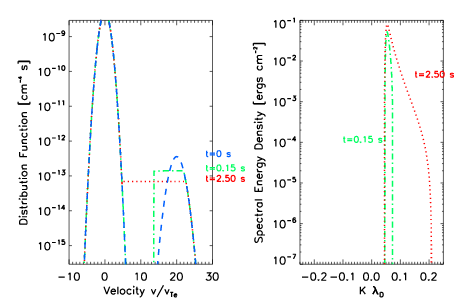
\includegraphics[width=0.75\columnwidth]{Images/L_wave_growth.png}
    \caption[Langmuir wave distriburtion function and spectral energy density.]{Left: Evolution of distribution function (normalised by the electron thermal velocity $v_{Te}=V_e$) in time. The diffusive term in \ref{eq:dfdt} causes the bump-on-tail Gaussian to turn into a plateau, thereby eliminating the instability caused by the positive velocity gradient. Right: The spectral energy density of generated Langmuir waves, x-axis normalised to the Debye length $\lambda_D=\sqrt{\frac{\epsilon_0 k_B T_e}{e^2 n_e}}$. As time passes the spectral range of Langmuir waves increases. Each panel shows successive times of t=0.15s (green, dot-dashed line) and t=2.50s (red, dotted line). \citep[Figure taken from][]{Reid2014}.} %(Figure taken from \citeauthor{Reid2014} \citeyear{Reid2014})}
    \label{fig:Lwavegrowth}
\end{figure}

\subsection{Wave-Wave Interaction}\label{Plasma Emission}
Wave-wave interaction concerns the processes by which three types of waves interact. These are: transverse (T) waves, Langmuir (L) waves and ion sound (S) waves, and have the following, respective dispersion relations,
$$ \omega=(\omega_p^2 +k^2c^2)^{\frac{1}{2}} $$
$$ \omega \cong \omega_p + \frac{3k^2V_e^2}{2 \omega_p}$$
$$ \omega = kv_s $$
where $V_e$ is the thermal velocity of electrons in the plasma, $v_s$ is the ion sound speed and $k$ is the wave vector. Only transverse waves with $\omega > \omega_p $ can escape and thus a plasma emission mechanism is a process that generates these transverse waves. 

As mentioned in Section \ref{characteristics}, Type III bursts have a harmonic structure associated with plasma emission at the plasma frequency and the second harmonic. Both of these transverse waves are formed in different three wave processes that will now be discussed.
In a plasma, due to scattering from other wave modes and ions in the plasma, a wave mode can be changed from one to the other. This is expressed in the equation 
$$ \sigma \rightleftarrows \sigma' + \sigma '' $$
where $\sigma$, $\sigma'$  and  $\sigma ''$ represent different wave modes. Conservation of energy and momentum state,
$$ \omega^{\sigma}(k)=\omega^{\sigma'}(k')+\omega^{\sigma''}(k'')$$
$$ k=k'+k''$$
where $ \omega^{\sigma}(k)$ is the frequency of a particular wave mode with the wave vector $k$. For Langmuir (L), ion sound (S) and transverse (T) wave modes the allowed processes are L+S$\rightarrow$L', L+S$\rightarrow$T,  T+S$\rightarrow$L,  T+S$\rightarrow$T' and  L+L'$\rightarrow$T. Of these L+S$\rightarrow$T,  L$\rightarrow$T+S are responsible for fundamental emission while harmonic emission is associated with the three wave process L+L'$\rightarrow$T.

Originally \cite{Ginzburg1958} considered fundamental emission to be due to Langmuir waves scattering off of thermal ions in the plasma. It is now commonly accepted that the biggest cause of fundamental emission is due to the three wave processes of a Langmuir wave coalescing with an ion sound wave generated by L$\rightarrow$L'+S or when a Langmuir wave decays into an ion sound wave and an electromagnetic transverse wave. The process L$\rightarrow$T+S can be visualised as in Figure \ref{fig:Femission}. In solar radio physics it is often assumed that $k_L \gg k_T$, knowing this and that the wave vectors must satisfy $\mathbf{k}_L \pm \mathbf{k}_s = \mathbf{k}_T$ ($+$ for L+S$\rightarrow$T , $-$ for L$\rightarrow$T+S) implies $\mathbf{k}_s \approx \mp \mathbf{k}_L$ 

\begin{figure}
\centering
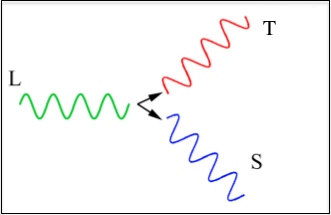
\includegraphics[width=0.5\columnwidth]{Images/Fundamental_emission_Lwaves.png}
\caption[A three wave process of fundamental plasma emission L$\rightarrow$T+S]{A three wave process of fundamental plasma emission L$\rightarrow$T+S. A Langmuir wave decaying into an ion sound wave and an electromagnetic transverse wave at the plasma frequency. (Figure adapted from Solar (interplanetary) Radio Bursts: the Generation of Radio Waves,	an oral presentation by David Malaspina at the Jean Louis Steinberg International Workshop on Solar, Heliospheric and Magnetospheric Radioastronomy, November 2017)}
\label{fig:Femission}
\end{figure}

Second harmonic emission occurs when two Langmuir waves coalesce in the process L+L'$\rightarrow$=T, shown in Figure \ref{fig:Hemission}. Conservation of momentum requires that $\mathbf{k}_L + \mathbf{k'}_L = \mathbf{k}_T$ and for second harmonic (H) generation, $k_T=k_H \approx \frac{\sqrt{3} \omega_p}{c}$. The phase speed $v_\phi$ of Langmuir waves is much less than $\frac{c}{\sqrt{3}}$ meaning that $k_L \gg k_T$ which results in $\mathbf{k}_L \approx -\mathbf{k'}_L$. This means that for a transverse wave at the second harmonic to be created, two Langmuir waves must coalesce almost exactly head on. These backward propagating Langmuir waves are generated: in the three wave processes of L+S$\rightarrow$L' and L$\rightarrow$L'+S; scattering off of thermal ions; and refraction at density inhomogeneities.
 \begin{figure}

     \centering
     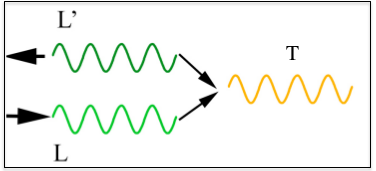
\includegraphics[width=0.5\columnwidth]{Images/Harmonic_emission_Lwaves.png}
     \caption[Three wave process of second harmonic plasma emission L+L' $\rightarrow$ T]{Three wave process of second harmonic plasma emission L+L' $\rightarrow$ T. A Langmuir wave (L) and a backwards propagating Langmuir wave (L') coalesce to form a transverse wave (T) at $2 \omega_p$. (Figure adapted from Solar (interplanetary) Radio Bursts: the Generation of Radio Waves,	an oral presentation by David Malaspina at the Jean Louis Steinberg International Workshop on Solar, Heliospheric and Magnetospheric Radioastronomy, November 2017)}
     \label{fig:Hemission}
 \end{figure}